\section{しりとり自己紹介(アイスブレイク)}
\subsection{日時・場所}
日時:2019年4月6日(土)09:00〜09:20\\
\ \ \ 場所:体育館\\

\subsection{目的}
名前を覚え,次のゲームを円滑に進めるため.お互いが打ち解け,話しやすい空気を作る.
\subsection{イベント内容(概要)}
自己紹介をしりとり形式で行う.8人で一つのグループになり,円に並ぶ.最初の人は司会が50音からランダムで出す一文字から自己紹介をはじめ,次の人は
前の人の名前の文字の中から一つ好きな文字を選んで自己紹介をする.\\
\ \ \ 例えば,名前が「山田太郎」の場合,「や」を選ぶと「ヤギが好きな田中広輔です。」と自己紹介をする。その場合「田中広輔」の中から始める.
\subsection{タイムスケジュール}
\begin{longtable}{p{3zw}p{39zw}}
    09:00 & \textbf{◎ 整列} \\
          & \ \ \textbullet \ \ 各スタッフは整列完了後,その場に座る\\
          & \ \ \textbullet \ \ 次の仕事を控えたスタッフは準備に入る\\
          & \ \ \textbullet \ \ 整列を終え,全員が座ったら頃合いを見て総合司会(新川,貞松)は話し始める\\

    09:03 & \textbf{◎ アイスブレイクの説明} \\
          & \ \ \textbullet \ \ 総合司会はイベント司会(伊崎,青山)にマイクを譲りパワーポイントを用いてアイスブレイクの説明を行う\\

    09:10 & \textbf{◎ しりとり自己紹介の説明} \\
          & \ \ \textbullet \ \ パワーポイントを用いてしりとり自己紹介の説明を行う\\
          & \ \ \textbullet \ \ 分からない新入生がいたら各班スタッフが補足説明を行う\\

    09:15 & \textbf{◎ しりとり自己紹介の開始} \\
          & \ \ \textbullet \ \ 司会が時間を5分計る\\

    09:20 & \textbf{◎ アイスブレイクを終了し休憩(10分間)} \\
          & \ \ \textbullet \ \ スタッフは9:30に再開することを伝え,トイレに行きたい新入生がいたら場所を伝える \\
\end{longtable}

\newpage

\subsection{必要物品}
\begin{itemize}
  \item ワイヤレスマイク:2個(司会用)
  \item スピーカー:2個
  \item 机:3個
  \item 椅子:1つ
  \item プロジェクター:2個(1個は幡多)
  \item スクリーン:2個
  \item PC
  \item カメラ

\end{itemize}
\subsection{備考}

\subsection{全体配置}
\begin{center}
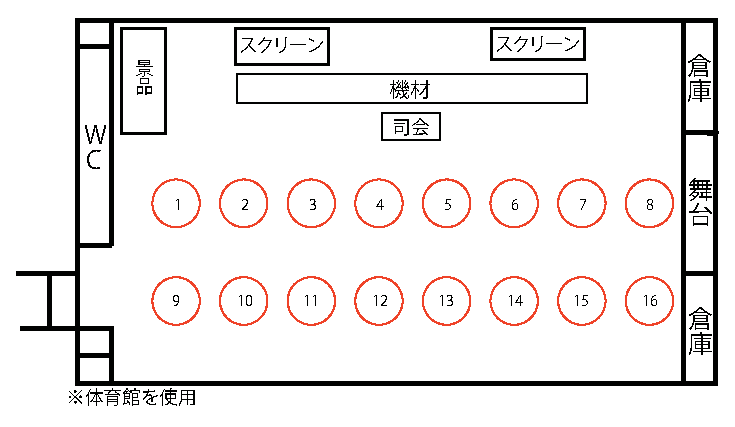
\includegraphics[width=12cm]{./21/reiout1.eps}
\label{fig:ice}

\end{center}
